\documentclass[journal,twoside,web]{ieeecolor}
\usepackage{generic}
\usepackage{cite}
\usepackage{amsmath,amssymb,amsfonts}
\usepackage{algorithmic}
\usepackage{graphicx}
\usepackage{textcomp}
 \usepackage{array,multirow,graphicx}
\definecolor{light-gray}{gray}{0.95}
\newcommand{\code}[1]{\colorbox{light-gray}{\texttt{#1}}}

\def\BibTeX{{\rm B\kern-.05em{\sc i\kern-.025em b}\kern-.08em
    T\kern-.1667em\lower.7ex\hbox{E}\kern-.125emX}}
\markboth{\journalname, VOL. XX, NO. XX, XXXX 2017}
{Author \MakeLowercase{\textit{et al.}}: Weka for Feature Selection and Its Application for Energy Efficiency in Smart Buildings}
\begin{document}
\title{Weka for Feature Selection and Its Application for Energy Efficiency in Smart Buildings}
\author{First A. Author, \IEEEmembership{Fellow, IEEE}, Second B. Author, and Third C. Author, Jr., \IEEEmembership{Member, IEEE}
\thanks{This paragraph of the first footnote will contain the date on 
which you submitted your paper for review. It will also contain support 
information, including sponsor and financial support acknowledgment. For 
example, ``This work was supported in part by the U.S. Department of 
Commerce under Grant BS123456.'' }
\thanks{The next few paragraphs should contain 
the authors' current affiliations, including current address and e-mail. For 
example, F. A. Author is with the National Institute of Standards and 
Technology, Boulder, CO 80305 USA (e-mail: author@boulder.nist.gov). }
\thanks{S. B. Author, Jr., was with Rice University, Houston, TX 77005 USA. He is 
now with the Department of Physics, Colorado State University, Fort Collins, 
CO 80523 USA (e-mail: author@lamar.colostate.edu).}
\thanks{T. C. Author is with 
the Electrical Engineering Department, University of Colorado, Boulder, CO 
80309 USA, on leave from the National Research Institute for Metals, 
Tsukuba, Japan (e-mail: author@nrim.go.jp).}}

\maketitle

\begin{abstract}


The massive collection of data via emerging technologies like the Internet of Things (IoT) requires finding optimal ways to
reduce the created features that have a potencial impact on the information that can be extracted through the machine learning process.

The mining of knowledgde related to a concept is done on the basis of the feature of the data. The process of finding the best combination of features in called feature extraction.


Different type of feature extraction methods are being used. The
feature selection algorithm should fit with the offline as weil as
on-line mining





\end{abstract}

\begin{IEEEkeywords}
feature selection, energy efficiency, smart buildings, smart cities
\end{IEEEkeywords}

\section{Introduction}
\label{sec:introduction}

Feature Selection (FS) is defined in~\cite{Liu:1998:FSK:551944} as the process of eliminating features from the data base that are irrelevant to the task to be performed. It should not be confused with Feature Extraction or Dimensionality Reduction, where new features are created combining the previous.
FS facilitates data understanding, reduces the measurement and storage requirements, reduces the computational process time, and reduces the size of a data set,  so that model learning becomes an easier process. It also avoids the curse of dimensionality (figure explaining xxx) 

A FS method can be seen as the combination of a search strategy for proposing feature subsets with a given evaluator that measures the performance of such candidates. The search space for candidate subsets has cardinality $O(2^w)$, where $w$ is the number of features. A stopping criterion establishes when the feature selection process must finish. Such criterion can be defined as a control procedure that ensures that no further addition or deletion of features does produce a better subset, or it can be as simple as a counter of iterations. 

FS methods are typically categorized into \textit{wrapper\textit{}}, \textit{filter} and \textit{embedded}, \textit{univariate} and \textit{multivariate} methods. 
\begin{itemize}

\item Filter methods apply statistical measures to evaluate the set of attributes independtly \cite{Kar10, Hal98, Ami05}. Correlation with the output, mutual information and Fisher test are some examples. %data similarity, local discriminative information, or data
reconstruction error
\item Wrapper methods \cite{kohavi1997wrappers} use a predetermined learning algorithm to determine the quality of selected features according to an evaluation metric \cite{Japkowicz:2011:ELA:1964882}.
\item Embedded methods take advantage of their own variable selection process and perform feature selection and model fitting simultaneously \cite{Sal94}.
\item  Multivariate methods evaluate features in batches.
\item  Univariate methods evaluate each feature independently.
\end{itemize}

The flow that characterises feature selection is depicted in Fig. \ref{fig:flow}


\begin{figure*} \label{fig:flow}
\centerline{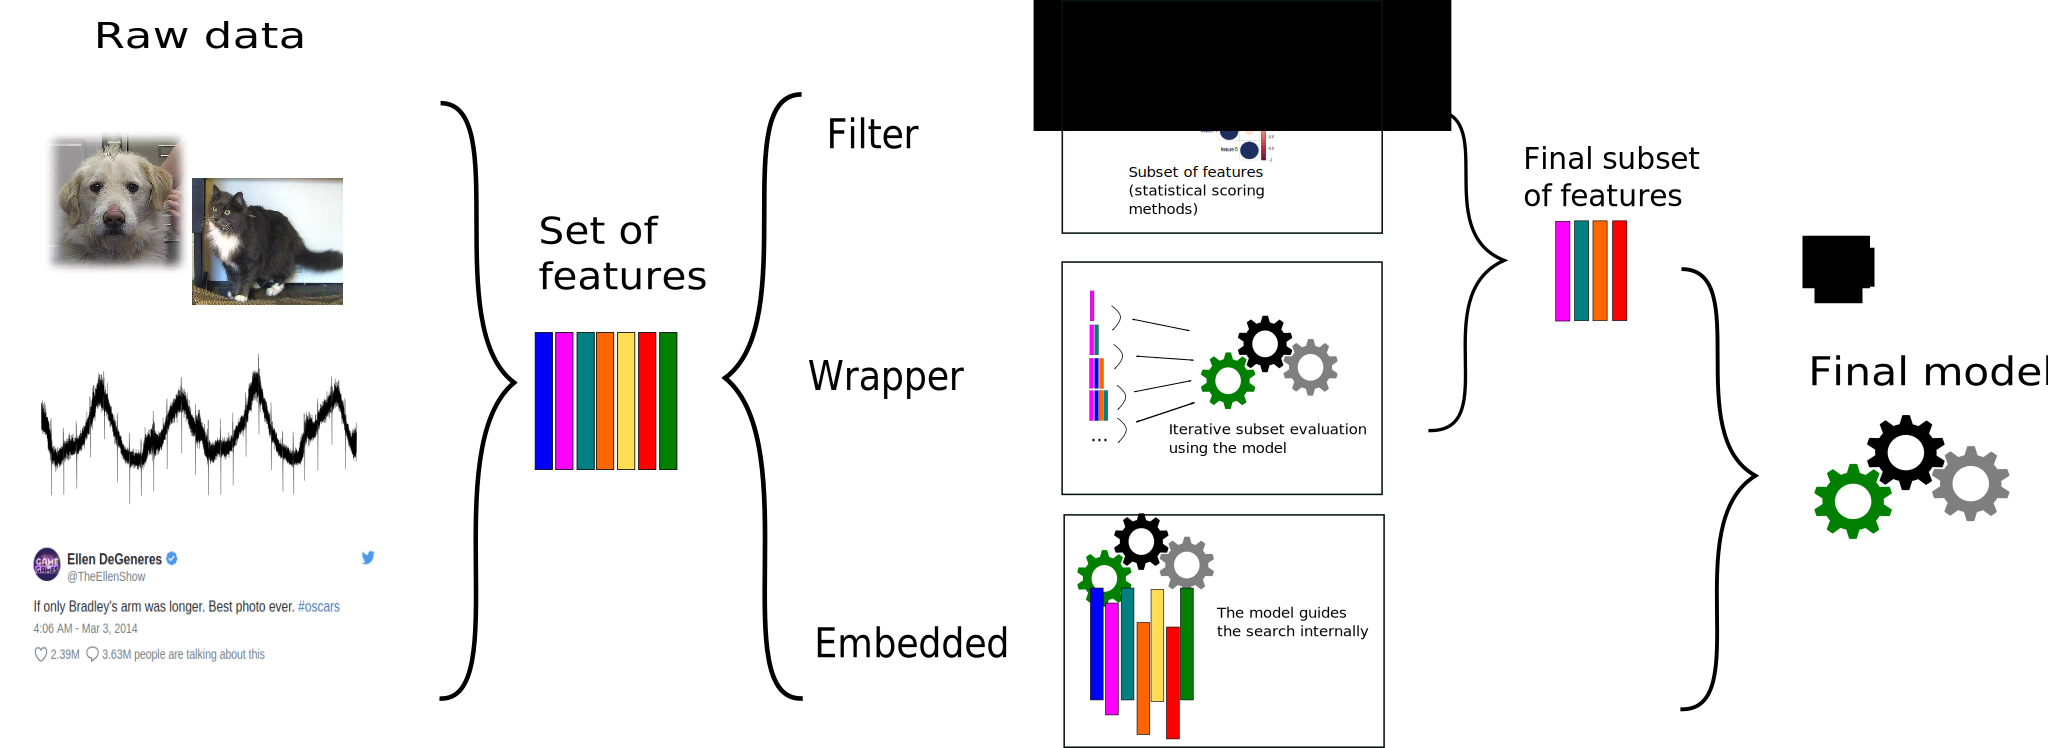
\includegraphics[width=16cm,height=16cm,keepaspectratio]{./creando_figs/drawing-ii.pdf}}
\caption{The feature selection flow}
\end{figure*}

Filter methods do not incorporate learning. Wrapper methods use a learning machine to measure the quality of subsets of features without incorporating knowledge about the specific structure of the classification or regression function, and can therefore be combined with any learning machine. In embedded methods the learning part and the feature selection part can not be separated, for example, Weston et al. [2000] measure the importance of a feature using a bound that is valid for Support Vector Machines only thus it is not possible to use this method with other models.



\subsection{Abbreviations and Acronyms}

Feature Selection: FS


\section{Feature Selection in Weka}

The free software licensed suite Waikato Environment for Knowledge Analysis (Weka) \cite{Weka} contains a collection of visualization tools and algorithms for data analysis and predictive modeling, together with graphical user interfaces for easy access to these functions.


In Weka, FS is implemented with the \\ \code{weka.attributeSelection} (w.aS) \\ package using two components of the \\\code{w.aS.AttributeSelection} (w.aS.AS) \\ class : the search strategy (\code{w.aS.ASSearch} abstract class) and the evaluators (\code{w.aS.ASEvaluation} abstract class). 


This structure allows users and programmers to configure a multitude of different methods for FS, both filter and wrapper, univariate and multivariate. 

Univariate methods are configured by evaluators with names ending in \textit{AttributeEval} and multivariate methods are configured by evaluators with names ending in \textit{SubsetEval}.

For multivariate wrapper FS methods, the \textit{w.aS} package has the \\ \code{w.aS.AS.WrapperSubsetEval} \\ class which evaluates attribute sets by using a learning scheme with  cross-validation and a performance measure. 

For univariate wrapper FS methods, the \\ \code{w.aS.AS.Classi\-fierAttributeEval} \\ class evaluates the worth of an attribute by using a user-specified classifier, cross-validation and a performance evaluation measure to use for selecting attributes. 

Since the FS and classification processes must be executed in bach mode, Weka offers the class
\\ \scriptsize \code{weka.classifiers.meta.AttributeSelected\-Classifier} \normalsize 
\\ which is a meta-classifier where dimensionality of data is reduced by attribute selection before being passed on to a learning algorithm.

¿Y QUÉ PASA CON LOS FILTER? xxx


\section{Weka FS Algorithms. Methodology}

In this section we analyse the search strategies, evaluators, regression methods and performance metrics that have been considered.

\subsection{Search strategies}

The search strategy will determine an interesting feature subset to train the model.

For univariate FS methods, \textit{Ranker} method \cite{yujor} is required. \textit{Ranker} method ranks attributes by their individual evaluations. A threshold, or the number of attributes to retain, allows reducing the attribute set.

xxx mete rollo sobre ranker

For multivariate FS methods, there exist two approaches: deterministic search  strategies (which xxx) and probabilistic algorithms.

\begin{itemize}

\item Deterministic search strategies: Greedy Stepwise \cite{russell2003modern}.

\code{GreedyStepwise} performs a greedy forward or backward search through the space of attribute subsets, stopping when the addition (forward direction) or deletion (backward direction) of any of the remaining attributes results in a decrease in evaluation, thus, it has no backtracking capability.

\item Probabilistic algorithms: \\ \code{MultiObjectiveEvolutionarySearch} \cite{jimenez2016multi} \\ and \code{PSO\-Search} \cite{moraglio2008geometric}.

\end{itemize}

\code{MultiObjectiveEvolutionarySearch}  uses evolutionary computation where two objectives are optimized: the first one is chosen by the evaluator, and it is to be maximized, while the second one is the attribute subset cardinality, and it is to be minimized. The final output is given by the non-dominated solutions in the last population having the best fitness score for the first objective.


\code{PSO} optimizes a problem moving individuals (particles) around in the search-space according to the particle's position and velocity, influenced by its local best known position and the best known positions.


\subsection{Evaluators}
%	\item[Evaluators] 

The subsets of features are evaluated in order to know whether they are interesting or the search must continuate.
	
	We considered the  multivariate filter evaluator   \emph{ConsistencySubsetEval} \cite{liu1996probabilistic}.  \emph{ConsistencySubsetEval}  sco\-res a subset of features as a whole, by projecting the training instances according to the attribute subset, and considering the consistency of class values in the obtained instance sets. As far as univariate filter evaluators are concerned, \textit{RelieffAttributeEval} \cite{Kira:1992:PAF:141975.142034} and \textit{PrincipalComponents} \cite{WICS:WICS101}  were considered. \textit{RelieffAttributeEval} evaluates the worth of an attribute by repeatedly sampling an instance and considering the value of the given attribute for the nearest instance of the same and different class. Can operate on both discrete and continuous class data. \textit{PrincipalComponents} performs a principal components analysis and transformation of the data.  Dimensionality reduction is accomplished by choosing enough eigenvectors to account for some percentage of the variance in the original data (default 95\%). Attribute noise can be filtered by transforming to the principal components space, eliminating some of the worst eigenvectors, and then transforming back to the original space.
		
	We use the wrapper \textit{WrapperSubsetEval}  \cite{kohavi1997wrappers} for multivariate FS methods and \textit{ClassifierAttributeEval} \cite{Schaefer2016b} for univariate FS methods 
	
\subsection{Models and metrics}

Wrapper methods are used in conjunction with the predictors \emph{RandomForest}~\cite{breiman2001random}, \emph{IBk}~\cite{Aha:1991:ILA:104713.104717} and \textit{LinearRegression} \cite{yan2009linear}, and with the metrics \emph{root mean squared error} (\textit{RMSE}) and \textit{mean absolute error} (\textit{MAE}) \cite{Willmott200579} both in univariate and multivariate scenarios. 

{\em RandomForest} is an \emph{ensemble learning} method which constructs a forest of random trees with controlled variance, for classification or regression purposes. {\em IBk} is a simple instance-based learner that uses the class of the nearest k training instances for the class of the test instances and it is also valid for regressión. \textit{LinearRegression} uses the \textit{Akaike} criterion for model selection, and is able to deal with weighted instances.

\begin{figure}[h!]
	
	\begin{center}
		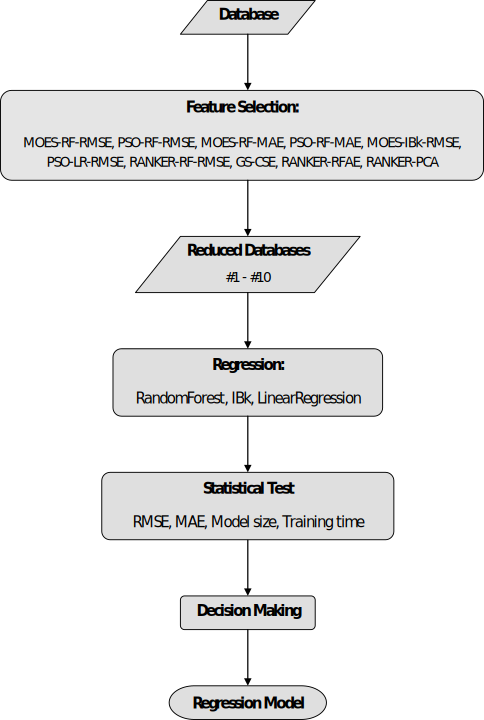
\includegraphics[scale=0.55]{./figs/metodology-i.pdf}
		\caption{Methodology for Feature Selection for regression.}
		\label{fig:grafico-metod} 
	\end{center}
\end{figure}


We have followed the methodology shown in the Figure \ref{fig:grafico-metod} to perform FS. We have systematically applied 10 different FS methods for regression shown in Table \ref{FSM} and graphically in Figure \ref{fig:FSmethods}. In Table \ref{FSM}, \textit{Database \#Id} denotes the identifier of the reduced database generated with each FS method. Each FS method is the result of a specific choice among the search strategy, the evaluator, and the performance metric (for wrapper FS methods). We considered for this research seven wrapper FS methods and three filter FS methods. Among them, seven FS methods are multivariate and three FS methods are univariate. Table \ref{PFSM} shows the parameters used for each FS method.



\begin{table*}[t]
  \centering
  \begin{tabular}{ccccc}
  	\textit{\textbf{Database \#Id.}} & \textit{\textbf{FS method}} & \textit{\textbf{Name}} & \textit{\textbf{Search strategy}} & \textit{\textbf{Evaluator}} \\\hline
	
	\textit{\#1} & Wrapper Multivariate & \textit{MOES-RF-RMSE} & \textit{MultiObjectiveEvolutionarySearch} & \textit{RandonForest (RMSE)}  \\
	\textit{\#2} &  Wrapper Multivariate & \textit{PSO-RF-RMSE} & \textit{PSOSearch} & \textit{RandonForest (RMSE)}  \\
	\textit{\#3} & Wrapper Multivariate & \textit{MOES-RF-MAE} & \textit{MultiObjectiveEvolutionarySearch} & \textit{RandonForest (MAE)}  \\	

	\textit{\#4} & Wrapper Multivariate & \textit{PSO-RF-MAE} & \textit{PSOSearch} & \textit{RandonForest (MAE)}  \\
	\textit{\#5} & Wrapper Multivariate & \textit{MOES-IBk-RMSE} & \textit{MultiObjectiveEvolutionarySearch} & \textit{IBk (RMSE)}  \\	
	\textit{\#6} & Wrapper Multivariate & \textit{PSO-LR-RMSE} & \textit{PSOSearch} & \textit{LinearRegression (RMSE)}  \\
	\textit{\#7} &  Wrapper Univariate & \textit{RANKER-RF-RMSE} & \textit{Ranker} & \textit{RandonForest (RMSE)}  \\
	\textit{\#8} &  Filter Multivariate & \textit{GS-CSE} & \textit{GreedyStepwise} & \textit{ConsistencySubsetEval}  \\
	\textit{\#9} &  Filter Univariate & \textit{RANKER-RFAE} & \textit{Ranker} & \textit{ReliefFAttributeEval}  \\
	\textit{\#10} &  Filter Univariate & \textit{RANKER-PCA} & \textit{Ranker} & \textit{PrincipalComponents}  \\
   \hline		
  \end{tabular}
	\caption{Proposed Feature Selection methods for regression.}
	\label{FSM}
	
	\end{table*}

\section{Use Case: Energy Efficiency}

Feature Selection is part of the analytics process and there is an enormous quantity of use cases where is applied nowadays. Almost in any scenario where machine learning is used, feature selection is involved.

For this work, we are going to compare the results on energy consumption prediction scenarios using Weka feature selection approach and the ones that we have carried out in previous works in order to asses the suitability of the discussed Weka feature selection process.

Energy consumption in buildings is of special interest since they are one of the largest consumers of primary energy; for example in European Union countries, energy consumption in buildings represents around 40\% of the total energy consumption. Attaining their efficiency is, therefore, an important goal since it can yield economical savings, reduce greenhouse gas emissions and alleviate energy poverty \cite{Gonzalez2017}.

The reference building in which the proposed procedure has been carried out in order to select features for generating accurate building models is the Chemistry Faculty of the University of Murcia, which is a building used as a pilot for the H2020 ENTROPY project\footnote{http://entropy-project.eu/}.  

The data that is used in order to build and train our baseline corresponds to 1 year's worth of data, from February 2016 to February 2017. 


\subsection{Considered Features}

Weather and the working hours have been proved to be useful in the task of energy consumption prediction \cite{gonzalez2016towards}.

However, due to the big amount of data that is available nowadays, the decision of which data source to use is reduced to the scientist subjective perception.

Not only there are three meteorological stations surrounding the Chemistry Faculty building, but also there exists many online services and API such as Weather Underground that might incorporate both more information but also more instability to the system. 


\subsection{Other Approaches}

xxx

\begin{itemize}

\item PCA - por tramos (mañana tarde y noche)

\cite{gonzalez2016towards}

\item MIC - por horas y por semanas

\cite{Vantuch2018}

\item Raw data - por días

\cite{Gonzalez2017}

\end{itemize}



%\clearpage

\subsection{Weka Feature Selection Results}

For this study, there are 51 features that have been studied.

Descríbelas xxx: unas vienen de IMIDA otras del Weather Underground


Once FS is made, the next step is to perform regression with the reduced and original databases using \textit{RandomForest}, \textit{IBk} and \textit{LinearRegression}. The Table \ref{PRM} shows the parameters used for the regression methods. In order to detect over-fitting and prediction ability, the regression models have been evaluated in both full training set and 10-fold cross-validation over 10 iterations. Tables \ref{RFTS} and \ref{MFTS} show the evaluation in full training set for the \textit{RMSE} and \textit{MAE} metrics respectively. The Tables\ref{RMCV}, \ref{SMSCV} and \ref{RTCV}
show the evaluation in 10-fold cross-validation (10 iterations) for the metrics \textit{RMSE}, \textit{MAE}, \textit{Serialized\_Model\_Size} and \textit{UserCPU\_Time\_testing}\footnote{Intel (R) Core (TM) i5-4460 @ 3.20 GHz 3.20 GHz RAM 8.00 GB Operating Systems 64 bits, processor x64.} respectively. The result of the experiment has been analysed through a \textit{paired t-test (corrected)},
with 0.05 significance (being \textit{\#1\#2} 
the test base in Tables \ref{MCV}, and \textit{RandomForest} in Tables \ref{SMSCV} and \ref{RTCV}). For each result, a mark $*$ denotes that the
result is statistically worse than the test base; similarly, a
mark $v$ denotes a statistically better result, and no mark denotes no statistically meaningful difference. Note that the reduced databases \textit{\#1} and \textit{\#2} are the same, as are the reduced databases \textit{\#3} and  \textit{\#4}, so they appear together in all the tables.

\begin{table}[h]
	\begin{center}
			\footnotesize{\begin{tabular}{cc}\hline
			\textit{\textbf{Name}} & \textit{\textbf{Parameters}} \\\hline
			
			\textit{RandomForest} & -P 100 -I 500 -num-slots 1 -K 0 -M 1.0 -V 0.001 -S 1\\
			\textit{IBk} & weka.classifiers.lazy.IBk -K 1 -W 0 \\
			& -A ``weka.core.neighboursearch.LinearNNSearch \\
			& -A ``weka.core.EuclideanDistance -R first-last""\\
			\textit{LinearRegression} & -S 0 -R 1.0E-8 -num-decimal-places 4\\\hline		
		\end{tabular}}
	\end{center}
	\caption{Parameters of the regression methods.}
	\label{PRM}
\end{table}	

\begin{table}[h]
	\begin{center}
			\footnotesize{\begin{tabular}{cccc}\hline
			\textit{\textbf{Database \#Id.}} & \textit{\textbf{RandomForest}} & \textit{\textbf{IBk}} & \textit{\textbf{LinearRegression
					}} \\\hline
			
		\textit{\#1\#2} & 4.2267 & 0.0 & 66.8625 \\	
		\textit{\#3\#4} & 4.2734 & 15.8069 & 66.8642 \\	
		\textit{\#5} & 4.6102 & 0.0 & 69.5321 \\
		\textit{\#6} & 9.3867 & 0.0 &  54.7665\\
		\textit{\#7} & 5.8233 & 0.0 & 62.1653\\
		\textit{\#8} & 6.8531 & 0.0 & 56.583 \\
		\textit{\#9} & 10.9122 & 7.0239 & 56.5407\\
		\textit{\#10} & 16.6868 & 0.0 & 58.8544\\
		\textit{Original} & 10.0615 & 0.0 & 54.6545\\
			\hline		
		\end{tabular}}
	\end{center}
	\caption{\textit{RMSE} with full training set.}
	\label{RFTS}
\end{table}

\begin{table}[h]
	\begin{center}
			\footnotesize{\begin{tabular}{cccc}\hline
			\textit{\textbf{Database \#Id.}} & \textit{\textbf{RandomForest}} & \textit{\textbf{IBk}} & \textit{\textbf{LinearRegression
				}} \\\hline
				
				\textit{\#1\#2} & 2.2503 & 0.0 & 51.4108\\
				\textit{\#3\#4} & 2.2696 & 4.7964 & 51.3844 \\	
				\textit{\#5} & 2.438 & 0.0 & 53.8089\\
				\textit{\#6} & 5.8176 & 0.0 & 39.4351 \\
				\textit{\#7} & 3.273 & 0.0 & 44.8639 \\
				\textit{\#8} & 4.005 & 0.0 & 40.8774\\
				\textit{\#9} & 5.9238 & 1.5123 & 41.52\\
				\textit{\#10} & 10.892 & 0.0 & 41.2654\\
				\textit{Original} & 6.2188 & 0.0  & 39.3108\\
				\hline		
			\end{tabular}}
		\end{center}
		\caption{\textit{MAE} with full training set.}
		\label{MFTS}
	\end{table}
	
\begin{table*}[h]
	\begin{center}
		\footnotesize{
 \begin{tabular}{|c|l|r|r|r|r|r|r|r|r|r|}
 \hline
 & \multicolumn{1}{c|}{\textit{\textbf{Model}}} & \multicolumn{1}{c|}{\textit{\textbf{\#1\#2}}} & \multicolumn{1}{c|}{\textit{\textbf{\#3\#4}}} & \multicolumn{1}{c|}{\textit{\textbf{\#5}}} & \multicolumn{1}{c|}{\textit{\textbf{\#6}}} & \multicolumn{1}{c|}{\textit{\textbf{\#7}}} & \multicolumn{1}{c|}{\textit{\textbf{\#8}}} & \multicolumn{1}{c|}{\textit{\textbf{\#9}}} & \multicolumn{1}{c|}{\textit{\textbf{\#10}}} & \multicolumn{1}{c|}{\textit{\textbf{Original}}} \\
 \hline
 \parbox[t]{2mm}{\multirow{3}{*}{\rotatebox[origin=c]{90}{RMSE}}} & \textit{RandomForest}	& 11.00 &   11.02  &    12.23 * &   26.04 * &   16.13 * &   18.82 * &   24.02 * &   46.02 *  &  27.59 * \\
 & \textit{IBk}	& 21.17 &   40.04 * &  20.82 v &   37.06 * &  34.47 *  &  30.24 * &   39.08 * &   46.79 * &   36.95  * \\
 & \textit{LinearRegression}	& 66.89 &    66.88  &    69.55 * &   55.09 v &   62.28 v &   56.72 v &  56.66 v &   58.93 v &   55.31 v \\
 \hline
  \parbox[t]{2mm}{\multirow{3}{*}{\rotatebox[origin=c]{90}{MAE}}} & \textit{RandomForest}	& 5.19 &     5.15  &     5.70 * &   15.93 *  &   8.51 * &   10.64 * &   13.54 * &   29.98 * &   16.82 * \\
 & \textit{IBk}	& 10.19 &    19.91 * &    9.99 v  &  17.31 * &   16.17 * &   13.74 * &   20.07 * &   21.21 *  &  16.69 *\\
 & \textit{LinearRegression}	& 51.46 &    51.44  &    53.87 * &   39.71 v &   44.97 v &   40.99 v &   41.62 v &   41.35 v &   39.81 v\\	
 \hline
 \end{tabular}
	
			}
		\end{center}
		\caption{\textit{RMSE} and \textit{MAE} with 10-fold cross-validation (10 iterations).}
		\label{RMCV}
	\end{table*}




			
		

\begin{table}[h]
	\begin{center}
		\footnotesize{\begin{tabular}{cccc}\hline
				 & \textit{\textbf{RandomForest}} & \textit{\textbf{IBk}} & \textit{\textbf{LinearRegression
					}} \\\hline
					
\textit{\#1\#2} &   77954766.98 &     513355.60 v &   54118.52 v\\
\textit{\#3\#4} &   75704860.26 &     403181.80 v &   53715.00 v\\
\textit{\#5} &   79702492.83 &     319109.36 v &    6339.56 v\\
\textit{\#6} &   91655663.29 &    1321302.40 v &   57163.96 v\\
\textit{\#7} &   82474001.83 &     586730.40 v &   54166.12 v\\
\textit{\#8} &   83994700.42 &     759559.00 v  &   7235.44 v\\
\textit{\#9} &   87917552.94 &     539231.84 v  &   6418.92 v\\
\textit{\#10} &   103251437.55 &     539979.40 v &    7176.08 v\\
\textit{Original}  &  89395544.24 &    2128847.60 v &   58977.72 v\\
					\hline		
				\end{tabular}}
			\end{center}
			\caption{\textit{Serialized\_Model\_Size} with 10-fold cross-validation (10 iterations).}
			\label{SMSCV}
		\end{table}

\begin{table}[h]
	\begin{center}
		\footnotesize{\begin{tabular}{cccc}\hline
				& \textit{\textbf{RandomForest}} & \textit{\textbf{IBk}} & \textit{\textbf{LinearRegression
					}} \\\hline
					
\textit{\#1\#2} &   0.18 &   0.11 v &   0.00 v\\
\textit{\#3\#4} &   0.19&    0.09 v &   0.00 v\\
\textit{\#5} &   0.18 &   0.08 v &   0.00 v\\
\textit{\#6} &   0.26 &   0.23 v &   0.00 v\\
\textit{\#7}&   0.22 &   0.10 v &   0.00 v\\
\textit{\#8} &   0.23 &   0.13 v &   0.00 v\\
\textit{\#9} &   0.23 &    0.09 v &   0.00 v\\
\textit{\#10}&    0.23 &    0.10 v &   0.00 v\\
\textit{Original}  &  0.24 &   0.29 * &   0.00 v\\
					\hline		
				\end{tabular}}
			\end{center}
			\caption{\textit{UserCPU\_Time\_testing} with 10-fold cross-validation (10 iterations).}
			\label{RTCV}
		\end{table}




\begin{table}[h!]
	\begin{center}
		\footnotesize{\begin{tabular}{cc}\hline
			\textit{\textbf{Database \#Id.}} & \textit{\textbf{Parameters}} \\\hline
			
			\textit{\#1} &  -E ``weka.attributeSelection.WrapperSubsetEval \\
			& -B weka.classifiers.trees.RandomForest  -F 5 -T 0.01 -R 1 \\
			& -E DEFAULT -- -P 100 -I 10 -num-slots 1 -K 0 -M 1.0 -V 0.001 -S 1" \\
			& -S ``weka.attributeSelection.MultiObjectiveEvolutionarySearch \\ 
			& -generations 1000 -population-size 100 -seed 1 -a 0 "\\
			
			
			\textit{\#2} &  -E ``weka.attributeSelection.WrapperSubsetEval \\
			& -B weka.classifiers.trees.RandomForest -F 5 -T 0.01 -R 1 \\
			& -E DEFAULT -- -P 100 -I 10 -num-slots 1 -K 0 -M 1.0 -V 0.001 -S 1" \\
			& -S ``weka.attributeSelection.PSOSearch -N 20 -I 1000 -T 0 \\
			&  -M 0.01 -A 0.33 -B 0.33 -C 0.34  -S 1"\\
			
			\textit{\#3} &  -E ``weka.attributeSelection.WrapperSubsetEval \\
			& -B weka.classifiers.trees.RandomForest  -F 5 -T 0.01 -R 1 \\
			& -E MAE -- -P 100 -I 10 -num-slots 1 -K 0 -M 1.0 -V 0.001 -S 1" \\
			& -S ``weka.attributeSelection.MultiObjectiveEvolutionarySearch \\ 
			& -generations 1000 -population-size 100 -seed 1 -a 0 "\\
			
			
			\textit{\#4} &  -E ``weka.attributeSelection.WrapperSubsetEval \\
			& -B weka.classifiers.trees.RandomForest -F 5 -T 0.01 -R 1 \\
			& -E MAE -- -P 100 -I 10 -num-slots 1 -K 0 -M 1.0 -V 0.001 -S 1" \\
			& -S ``weka.attributeSelection.PSOSearch -N 20 -I 1000 -T 0 \\
			&  -M 0.01 -A 0.33 -B 0.33 -C 0.34  -S 1"\\
			
			
			\textit{\#5} &  -E 
			 ``weka.attributeSelection.WrapperSubsetEval \\
			& -B weka.classifiers.lazy.IBk -F 5 -T 0.01 -R 1 \\
			& -E DEFAULT -- -K 1 -W 0 \\
			& -A ``weka.core.neighboursearch.LinearNNSearch \\
			& -A ``weka.core.EuclideanDistance -R first-last""  \\
			& -S ``weka.attributeSelection.MultiObjectiveEvolutionarySearch \\
			 & -generations 10 -population-size 100 -seed 1 -a 0" \\
			
			
			\textit{\#6} & -E ``weka.attributeSelection.WrapperSubsetEval \\
			& -B weka.classifiers.functions.LinearRegression -F 5 -T 0.01 -R 1 \\
			& -E DEFAULT -- -S 0 -R 1.0E-8 -num-decimal-places 4" \\
			& -S "weka.attributeSelection.PSOSearch -N 100 -I 1000 -T 0 \\
			& -M 0.01 -A 0.33 -B 0.33 -C 0.34 -R 1000 -S 1"\\
			
			
			\textit{\#7} & -E ``weka.attributeSelection.WrapperSubsetEval \\
			& -B weka.classifiers.trees.RandomForest -F 5 -T 0.01 -R 1 \\
			& -E DEFAULT -- -P 100 -I 10 -num-slots 1 -K 0 -M 1.0 -V 0.001 -S 1" \\
			& -S ``weka.attributeSelection.Ranker -T -1.8E308 -N 10"\\
			\textit{\#8} & -E ``weka.attributeSelection.CfsSubsetEval -P 1 -E 1" \\
			& -S ``weka.attributeSelection.GreedyStepwise -T -1.8E308 -N -1 -num-slots 1"\\
			\textit{\#9} & -E ``weka.attributeSelection.ReliefFAttributeEval -M -1 -D 1 -K 10" \\
			& -S "weka.attributeSelection.Ranker -T -1.8E308 -N 10"\\
			\textit{\#10} & -E ``weka.attributeSelection.PrincipalComponents -R 0.95 -A 5"\\
			& -S ``weka.attributeSelection.Ranker -T -1.8E308 -N 10"\\
			
			\hline		
		\end{tabular}}
	\end{center}
	\caption{Parameters of the Feature Selection methods for regression.}
	\label{PFSM}
\end{table}




\begin{figure*} \label{fig:dos}
\centerline{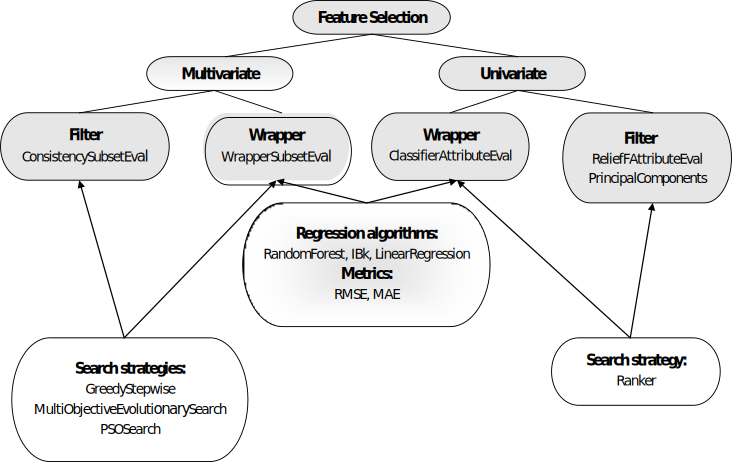
\includegraphics[scale=0.7]{./figs/FS-i.pdf}}
\caption{Organization chart of the proposed Feature Selection methods for regression.}\label{fig:FSmethods}
\end{figure*}

\section{Analysis of results and discussion}

Clearly the best results have been obtained with the FS methods \textit{MOES-RF-RMSE} / \textit{PSO-RF-RMSE} (\textit{\#1\#2}) and \textit{MOES-RF-MAE} / \textit{PSO-RF-MAE} (\textit{\#3\#4}), which show statistically significant differences with respect to the rest of the analysed FS methods for the \textit{RMSE} and \textit{MAE} performance metrics. The Table \ref{SA} show the selected attributes with these FS methods. All attributes of \textit{\#3\#4} also belong to \textit{\#1\#2}, and the performances of the databases are similar  in both full training set and 10-fold cross-validation (10 iterations).
We can then conclude that the best selection of attributes is the solution \textit{\#3\#4}.

\begin{table}[h]
	\begin{center}
			\footnotesize{\begin{tabular}{cc}\hline
		\textit{\textbf{Database \#Id.}} & \textit{\textbf{Attributes}} \\\hline
		\textit{\#1\#2} & time, hour, stMO12\_IMI\_prec, stMU62\_IMI\_prec, month, day, dow, holiday \\
		
		\textit{\#3\#4} & time, hour, day, dow, holiday \\\hline	
	\end{tabular}}
	\end{center}
	\caption{Best selected attributes.}
	\label{SA}
\end{table}


The following general statements can be derived from the results:

\begin{itemize}
	\item Wrapper FS methods have shown better performance for \textit{RMSE} and \textit{MAE} metrics than filter FS methods.
	\item Multivariate FS methods have shown better performance for \textit{RMSE} and \textit{MAE} metrics than univariate FS methods.
	\item For wrapper FS methods, \textit{RandomForest} has proven more effective than \textit{IBk} and \textit{LinearRegression} based evaluators. 
	\item Run time of \textit{RandomForest} is acceptable for wrapper FS methods setting the number of iterations to 10 (-I 10), and the method is not very sensitive to the variation of its parameters. However, \textit{RandomForest} generates large size regression models.
	\item \textit{IBk}  is very prone to over-fitting.
	
	\item \textit{LinearRegression} is very fast and not prone to over-fitting, but it has not been efficient for this problem.
	
\end{itemize}



\section*{Acknowledgment}



%\section*{References}

\bibliographystyle{elsarticle-num} 
\bibliography{references}

\clearpage
\begin{IEEEbiography}[{\includegraphics[width=1in,height=1.25in,clip,keepaspectratio]{a1.png}}]{First A. Author} (M'76--SM'81--F'87) and all authors may include 
biographies. Biographies are often not included in conference-related
papers. This author became a Member (M) of IEEE in 1976, a Senior
Member (SM) in 1981, and a Fellow (F) in 1987. The first paragraph may
contain a place and/or date of birth (list place, then date). Next,
the author's educational background is listed. The degrees should be
listed with type of degree in what field, which institution, city,
state, and country, and year the degree was earned. The author's major
field of study should be lower-cased. 

The second paragraph uses the pronoun of the person (he or she) and not the 
author's last name. It lists military and work experience, including summer 
and fellowship jobs. Job titles are capitalized. The current job must have a 
location; previous positions may be listed 
without one. Information concerning previous publications may be included. 
Try not to list more than three books or published articles. The format for 
listing publishers of a book within the biography is: title of book 
(publisher name, year) similar to a reference. Current and previous research 
interests end the paragraph. The third paragraph begins with the author's 
title and last name (e.g., Dr.\ Smith, Prof.\ Jones, Mr.\ Kajor, Ms.\ Hunter). 
List any memberships in professional societies other than the IEEE. Finally, 
list any awards and work for IEEE committees and publications. If a 
photograph is provided, it should be of good quality, and 
professional-looking. Following are two examples of an author's biography.
\end{IEEEbiography}

\begin{IEEEbiography}[{\includegraphics[width=1in,height=1.25in,clip,keepaspectratio]{a2.png}}]{Second B. Author} was born in Greenwich Village, New York, NY, USA in 
1977. He received the B.S. and M.S. degrees in aerospace engineering from 
the University of Virginia, Charlottesville, in 2001 and the Ph.D. degree in 
mechanical engineering from Drexel University, Philadelphia, PA, in 2008.

From 2001 to 2004, he was a Research Assistant with the Princeton Plasma 
Physics Laboratory. Since 2009, he has been an Assistant Professor with the 
Mechanical Engineering Department, Texas A{\&}M University, College Station. 
He is the author of three books, more than 150 articles, and more than 70 
inventions. His research interests include high-pressure and high-density 
nonthermal plasma discharge processes and applications, microscale plasma 
discharges, discharges in liquids, spectroscopic diagnostics, plasma 
propulsion, and innovation plasma applications. He is an Associate Editor of 
the journal \emph{Earth, Moon, Planets}, and holds two patents. 

Dr. Author was a recipient of the International Association of Geomagnetism 
and Aeronomy Young Scientist Award for Excellence in 2008, and the IEEE 
Electromagnetic Compatibility Society Best Symposium Paper Award in 2011. 
\end{IEEEbiography}

\begin{IEEEbiography}[{\includegraphics[width=1in,height=1.25in,clip,keepaspectratio]{a3.png}}]{Third C. Author, Jr.} (M'87) received the B.S. degree in mechanical 
engineering from National Chung Cheng University, Chiayi, Taiwan, in 2004 
and the M.S. degree in mechanical engineering from National Tsing Hua 
University, Hsinchu, Taiwan, in 2006. He is currently pursuing the Ph.D. 
degree in mechanical engineering at Texas A{\&}M University, College 
Station, TX, USA.

From 2008 to 2009, he was a Research Assistant with the Institute of 
Physics, Academia Sinica, Tapei, Taiwan. His research interest includes the 
development of surface processing and biological/medical treatment 
techniques using nonthermal atmospheric pressure plasmas, fundamental study 
of plasma sources, and fabrication of micro- or nanostructured surfaces. 

Mr. Author's awards and honors include the Frew Fellowship (Australian 
Academy of Science), the I. I. Rabi Prize (APS), the European Frequency and 
Time Forum Award, the Carl Zeiss Research Award, the William F. Meggers 
Award and the Adolph Lomb Medal (OSA).
\end{IEEEbiography}

\end{document}
\grid
\grid
\grid
\grid
\grid
